% !TEX TS-program = xelatex
%
\documentclass{beamer}

\usetheme{metropolis}

\usepackage{fontspec}
\defaultfontfeatures{Ligatures=TeX}

\usefonttheme{professionalfonts}
\usepackage[familydefault,light]{Chivo}

\usepackage{graphicx}

\usepackage{tkz-graph}
\tikzset{vertex/.style = {shape=circle,draw,minimum size=1}}
\tikzset{edge/.style = {->,> = latex'}}

\definecolor{red}{RGB}{200,50,0}
\definecolor{green}{RGB}{0,150,60}
\newcommand*{\red}{\color{red}}
\newcommand*{\green}{\color{green}}

\hypersetup
{
  pdftitle   = {Process Calculi for Concurrency},
  pdfauthor  = {Michael Kaltschmid \& Markus Reiter}
}

\title{Process Calculi}
\subtitle{for Concurrency}
\author{Michael Kaltschmid \& Markus Reiter}
\date{}

\begin{document}
  \maketitle

  \begin{frame}{Outline}
    \begin{itemize}
      \item What is a Process Calculus?
      \item µ-Calculus
      \item mCRL2
    \end{itemize}
  \end{frame}

  \begin{frame}{What is a Process Calculus?}
    \begin{itemize}
      \item approach for formally modelling concurrent systems
      \item tool for high-level description of interactions, communications and synchronizations between processes
      \item provides algebraic laws to allow analyzing and transforming process descriptions
      \item permits formal reasoning about equivalences between processes (e.g., using bisimulation)
    \end{itemize}
  \end{frame}

  \begin{frame}{Process Calculi}
    \begin{itemize}
      \item ACP
      \item CCS
      \item CSP
      \item Join-Calculus
      \item \textbf{µ-Calculus}
      \item PEPA
      \item π-Calculus
    \end{itemize}
  \end{frame}

  \begin{frame}{Labelled Transition Systems}
    \begin{itemize}
      \item Directed labelled graph \\
      \item Consists of a set of state and a set of transitions labelled with actions that connect the states \\
      \item Must have an initial state \\
      \item Deadlock if a reachable state does not terminate and has no outgoing transitions \\
    \end{itemize}
    \begin{tabular}{cc}
      \begin{minipage}{.5\linewidth}
        \centering
        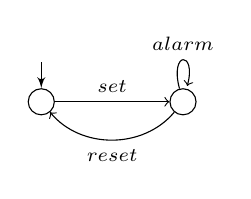
\begin{tikzpicture}[font=\sffamily\scriptsize]
          \node[vertex] (a) at (0, 0) {};
          \node[vertex] (b) at (1.8, 0) {};

          \draw[edge] (0, 0.5) to (a);
          \path[->] (a) edge  node[above] {$set$} (b);
          \path[->] (b) edge  [loop above] node {$alarm$} ();
          \path[->] (b) edge  [bend left=50] node[below] {$reset$} (a);
        \end{tikzpicture}
      \end{minipage}
      \begin{minipage}{.5\linewidth}
        \centering
        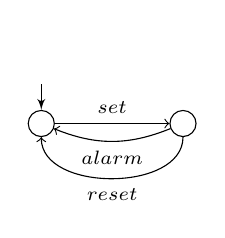
\begin{tikzpicture}[font=\sffamily\scriptsize]
          \node[vertex] (a) at (0, 0) {};
          \node[vertex] (b) at (1.8, 0) {};
          \node at (0, 1.1) {};

          \draw[edge] (0, 0.5) to (a);
          \path[->] (a) edge  node[above] {$set$} (b);
          \path[->] (b) edge  [bend left=22] node[below] {$alarm$} (a);
          \path[->] (b) edge  [bend left=90] node[below] {$reset$} (a);
        \end{tikzpicture}
      \end{minipage}
    \end{tabular}
  \end{frame}

  \begin{frame}{Labelled Transition Systems}
    LTS is a tuple $(S, A, \to,s_0>)$ where: \\[12pt]
    \begin{itemize}
      \item $S$ is a set of states \\
      \item $A$ is a set of actions \\
      \item $\to\ \subseteq S \times A \times S$ is a transition relation \\
      \item $s_0 \in S$ is the initial state \\
    \end{itemize}
  \end{frame}

  \begin{frame}{Hennessy-Milner Logic}
    \begin{align*}
      af ::= \alpha\ |\ true\ |\ false\ |\ \neg \phi\ |\ \phi \land \psi\ |\ \phi \lor \psi\ |\ \phi \to \psi\ |\ \langle a \rangle \phi \ |\ [a]\phi
    \end{align*}
    \begin{itemize}
      \item $\neg ,\ \land\ ,\ \lor$ as usual
      \item $\langle a \rangle \phi$ is valid whenever an $a-action$ can be performed such that $\phi$ is valid after this $a$ has been done
      \item $[a]\phi$ is valid when for every action $a$ that can be done, $\phi$ holds after doing that $a$
    \end{itemize}
  \end{frame}

  \begin{frame}{Fixed Point Modalities}
    By extending the Hennessy-Milner logic with fixed points we have:
    \resizebox{ \textwidth}{!} {
      \begin{minipage}{\textwidth}
        \begin{align*}
          af ::= \alpha\ |\ true\ |\ false\ |\ \neg \phi\ |\ \phi \land \psi\ |\ \phi \lor \psi\ |\ \phi \to \psi\ |\ \langle a \rangle \phi \ |\ [a]\phi\ |\ \color{green} \mu X. \phi \ |\ vX. \phi \ |\ X.
        \end{align*}
      \end{minipage}
    }
    \begin{itemize}
      \item $\mu X. \phi$ is the minimal fixed point
      \item $vX. \phi$ is the maximal fixed point
    \end{itemize}
  \end{frame}

  \begin{frame}{Diamond \& Box Modalities}
    \resizebox{\textwidth}{!}{
      \newcommand{\valid}{{\color{green} valid}}
      \newcommand{\invalid}{{\color{red} invalid}}
      \renewcommand{\arraystretch}{2}
      \begin{tabular}{l c c c c}
        &

        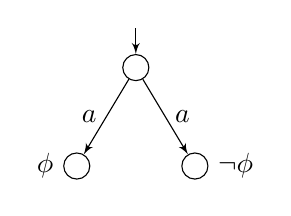
\begin{tikzpicture}
          \node[vertex] (a) at (0.75, 1.25) {};
          \node[vertex] [label=left:{$\phi$}] (b) at (0, 0) {};
          \node[vertex] [label=right:{$\neg\phi$}] (c) at (1.5, 0) {};

          \draw[edge] (.75, 1.75) to (a);
          \draw[edge] (a) to node [left] {$a$} (b);
          \draw[edge] (a) to node [right] {$a$} (c);
        \end{tikzpicture}

        &

        \begin{tikzpicture}
          \node[vertex] (a) at (0, 1.25) {};
          \node at (0, -0.175) {};

          \draw[edge] (0, 1.75) to (a);
        \end{tikzpicture}

        &

        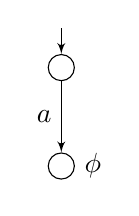
\begin{tikzpicture}
          \node[vertex] (a) at (0, 1.25) {};
          \node[vertex] [label=right:{$\phi$}] (b) at (0, 0) {};

          \draw[edge] (0, 1.75) to (a);
          \draw[edge] (a) to node [left] {$a$} (b);
        \end{tikzpicture}

        &

        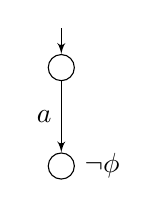
\begin{tikzpicture}
          \node[vertex] (a) at (0, 1.25) {};
          \node[vertex] [label=right:{$\neg\phi$}] (b) at (0, 0) {};

          \draw[edge] (0, 1.75) to (a);
          \draw[edge] (a) to node [left] {$a$} (b);
        \end{tikzpicture}

        \\

        $\langle{}a\rangle{}\phi$ & \valid   & \invalid & \valid & \invalid \\

        $[a]\phi$                 & \invalid & \valid   & \valid & \invalid \\
      \end{tabular}
    }
  \end{frame}

  \begin{frame}{Regular Formulae}
    \begin{itemize}
      \item allow more than a single action in a modality
      \item useful for expressing that after two or more \\
            arbitrary actions, a specific action must happen
      \item based on action formulae
    \end{itemize}

    \begin{exampleblock}{A more concrete example:}
      After two \textit{\textbf{receive}} actions, a \textit{\textbf{send}} action must follow.
    \end{exampleblock}
  \end{frame}

  \begin{frame}{Action Formulae}
    An action formula $af$ defines a set of multi-actions.

    \begin{align*}
      af ::= \alpha\ |\ true\ |\ false\ |\ \overline{af}\ |\ af\ \cap\ af\ |\ af\ \cup\ af
    \end{align*}

    \begin{itemize}
      \item $\alpha$ represents the set with exactly the multi-action $\alpha$.
      \item $true$ is the set of all multi-actions.
      \item $false$ is the empty set.
      \item $\overline{af}$ denotes the complement of the set $af$.
      \item $\cup$ and $\cap$ denote union and intersection, respectively.
    \end{itemize}
  \end{frame}

  \begin{frame}{Action Formulae}
    $af$ being a set of multi-actions, modalities with action formulae are defined like this:

    \begin{align*}
      \langle{af}\rangle\phi = \bigvee_{\alpha \in af} \langle\alpha\rangle\phi
      \qquad\qquad
      [af]\phi = \bigwedge_{\alpha \in af} [\alpha]\phi
    \end{align*}

    \begin{exampleblock}{Example}
      \begin{itemize}
        \item $\langle\overline{a}\rangle\langle{b \cup c}\rangle{true}$ means an action other than $a$ can be done, followed by either $b$ or $c$.
        \item $[\overline{a}]false$ says that only an $a$ action is allowed.
      \end{itemize}
    \end{exampleblock}
  \end{frame}

  \begin{frame}{Regular Formulae}
    Regular formulae extend action formulae, allowing sequences of actions in modalities.

    \begin{align*}
      R ::= \epsilon\ |\ af\ |\ R\cdot{R}\ |\ R+R\ |\ R^*\ |\ R^+
    \end{align*}

    \begin{itemize}
      \item $\epsilon$ is the empty sequence of actions.
      \item $R_1\cdot{R_2}$ represents the concatenation of $R_1$ and $R_2$.
      \item $R_1+R_2$ denotes the union of  $R_1$ and $R_2$.
      \item $R^*$ denotes zero ore more repetitions.
      \item $R^+$ denotes one ore more repetitions.
    \end{itemize}
  \end{frame}

  \begin{frame}{Regular Formulae}
    \begin{exampleblock}{Examples}
      \begin{itemize}
        \item $[\epsilon]\phi = \langle\epsilon\rangle\phi = \phi$, so one can always perform no action, and remain in the same state.
        \item $\langle{a}\cdot{b}\cdot{c}\rangle{true}$ is the same as $\langle{a}\rangle\langle{b}\rangle\langle{c}\rangle{true}$.
        \item $[a\cdot{b} + c\cdot{d}]false$ means that neither the sequence $a\cdot{b}$ nor $c\cdot{d}$ is possible.
        \item $\langle{a^*}\rangle{true}$ expresses that any sequence of $a$ actions is possible.
        \item $[a^+]\phi$ says that $\phi$ must hold in any state reachable by one or more $a$ actions.
      \end{itemize}
    \end{exampleblock}
  \end{frame}

  \begin{frame}{Regular Formulae}
    Two other commonly used formulae are the \textit{always} and \textit{eventually} modalities.

    \begin{align*}
      \square\phi = [true^*]\phi \qquad\qquad    \diamond\phi = \langle{true^*}\rangle\phi
    \end{align*}

    \begin{itemize}
      \item $\square\phi$ means that $\phi$ holds in all reachable states.
      \item $\diamond\phi$ says that there is a sequence of actions after which $\phi$ holds.
    \end{itemize}
  \end{frame}

  \begin{frame}{Regular Formulae}
    \begin{align*}
      \square\phi \implies \text{Something bad will never happen.}
    \end{align*}

    \begin{exampleblock}{Example}
      We have a program with a critical region and two actions, \textit{enter} and \textit{leave}.

      \begin{align*}
        [true^*\cdot enter \cdot \overline{leave}^* \cdot enter]false
      \end{align*}

      It is impossible to enter twice in a row. There has to be a \textit{leave} action in between two \textit{enter} actions.
    \end{exampleblock}
  \end{frame}

  \begin{frame}{Regular Formulae}
    \begin{align*}
      \diamond\phi \implies \text{Something good will happen.}
    \end{align*}

    \begin{exampleblock}{Example}
      \begin{align*}
        [true^*\cdot send]\langle true^* \cdot receive \rangle true
      \end{align*}

      Every time a message is sent, it can eventually be received.
    \end{exampleblock}
  \end{frame}
\end{document}
